%\documentclass[10pt]{beamer}
\documentclass[10pt,handout]{beamer}
\usepackage[english]{babel}
% % \usepackage[backend=biber, style=authoryear-icomp]{biblatex}
\resetcounteronoverlays{exx}
\usepackage{mdframed}
\usepackage{tikz}
\usepackage{blindtext}
\usepackage{tipa}
% \usepackage{cgloss4e}
% \usepackage{gb4e}
% \usepackage{qtree}
\usepackage{cancel}
\usepackage{wrapfig}
\usepackage{soul}
\usepackage{enumerate}
\usepackage{longtable}
\graphicspath{ {.} } % declaramos donde estan las imagenes
\usepackage[labelformat=simple]{subcaption} % para varias imagenes juntas
\renewcommand\thesubfigure{(\alph{subfigure})}
\usepackage[utf8]{inputenc}
\usepackage{amsmath}
\usepackage{amsfonts} % simbolos como el I de matriz identidad
\usepackage{bm}
\usepackage{graphicx} % paquete para ver imagenes
\usepackage{setspace}
\usepackage[T1]{fontenc}
\usepackage{parskip}
\usepackage{color}
\usepackage{framed}
\usetheme{Copenhagen}
\definecolor{frenchblue}{rgb}{0.0, 0.45, 0.73} % ESTE!!!!
\definecolor{myblue1}{RGB}{35,119,189}
\definecolor{myblue2}{RGB}{95,179,238}
\definecolor{myblue3}{RGB}{129,168,207}
\definecolor{myblue4}{RGB}{26,89,142}

\setbeamercolor{block body}{bg=frenchblue!50}
\setbeamercolor*{structure}{fg=frenchblue,bg=blue}
\setbeamertemplate{frametitle}[default][center]
\setlength{\parskip}{12pt}
\useoutertheme{infolines} % me comia mucho espacio de la otra fgorma
\makeatother
\setbeamertemplate{footline}
{
  \leavevmode%
  \hbox{%
  \begin{beamercolorbox}[wd=.3\paperwidth,ht=2.25ex,dp=1ex,center]{author in head/foot}%
    \usebeamerfont{author in head/foot}\insertshortauthor
  \end{beamercolorbox}%
  \begin{beamercolorbox}[wd=.6\paperwidth,ht=2.25ex,dp=1ex,center]{title in head/foot}%
    \usebeamerfont{title in head/foot}\insertshorttitle
  \end{beamercolorbox}%
  \begin{beamercolorbox}[wd=.1\paperwidth,ht=2.25ex,dp=1ex,center]{date in head/foot}%
    \insertframenumber{} / \inserttotalframenumber\hspace*{1ex}
  \end{beamercolorbox}}%
  \vskip0pt%
}
\newcommand{\floor}[1]{\lfloor #1 \rfloor}

\makeatletter
\setbeamertemplate{navigation symbols}{}
%\setbeameroption{show notes}
\setbeameroption{hide notes}


\usepackage{hyperref}

\title[CHACO]{Client-optimized Algorithms and Acceleration for Encrypted Compute Offloading \\
Part 1}
\author[Matias Mazzanti]{Matias Mazzanti}




\institute{}
\date{28 of March de 2023}


\begin{document}

\begin{frame}

\maketitle

\end{frame}


\section{Organization}
%%%%%%%%%%%%%%%%%%%%%%%%%%%%%%%%%%%%%%%%%%%%%%%%%%%%%%%%%%%%%%%%%%%%%%%%%%%%%%%%%%%%%%%%%%%%%%%%%%%%


\begin{frame}
    \frametitle{Schedule}

    \begin{itemize}
        \item What is HE?
        \item What is FHE?
        \item Schemes
        \item Math notation
    \end{itemize}


\end{frame}

%%%%%%%%%%%%%%%%%%%%%%%%%%%%%%%%%%%%%%%%%%%%%%%%%%%%%%%%%%%%%%%%%%%%%%%%%%%%%%%%%%%%%%%%%%%%%%%%%%%%
\begin{frame}
\frametitle{What is HE?}


    Homomorphic Encrpytion (HE) $\rightarrow$ form of encryption. Earlys 80s
\vspace{-0.3cm}

    Operate \textbf{directly} with encrypted data (without the need of decrypt).
\vspace{0.3cm}
  \begin{columns}
    \column{0.5\textwidth}
Typical use case:
\begin{itemize}
    \item Client encrypted his data with his own secret key.
    \item Send this and the public key to the server.
    \item Server operates with out decrypting (e.g. Machine Learning).
    \item Server send back the result in the encryption form.
    \item Client desencripts the result with the secret key.
\end{itemize}


\column{0.5\textwidth}

\begin{figure}[h!]
    \centering
    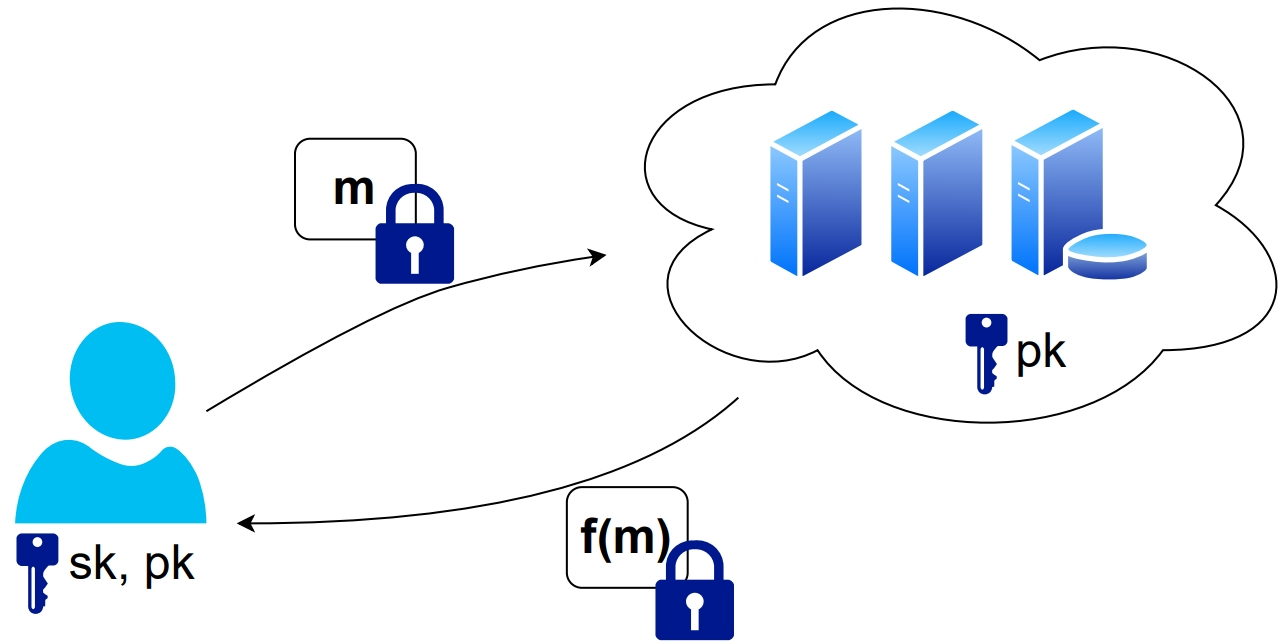
\includegraphics[scale=0.1]{fhe.jpg}
    \caption{Paper:https://ia.cr/2022/657}
\end{figure}
\end{columns}
 \vspace{-0.3cm}


Potentially very useful for cloud computing use.
 \vspace{-0.3cm}

 \pause
    \textbf{Present}: Orders of magnitude \textbf{slower} for real use.


\end{frame}

%%%%%%%%%%%%%%%%%%%%%%%%%%%%%%%%%%%%%%%%%%%%%%%%%%%%%%%%%%%%%%%%%%%%%%%%%%%%%%%%%%%%%%%%%%%%%%%%%%%%


\begin{frame}
    \frametitle{FHE}
  \begin{columns}
    \column{0.5\textwidth}
    In general, HE schemes use \texttt{Ring Learning With Errors} (RLWE) that  adds some sort of error to the encryption.

\vspace{0.3cm}
    This error grows in each operation (particulary wiht multiplications).

\vspace{0.3cm}
    If the error is too big the decrpytion will not work.
    \column{0.5\textwidth}
        \begin{figure}[h!]
            \centering
            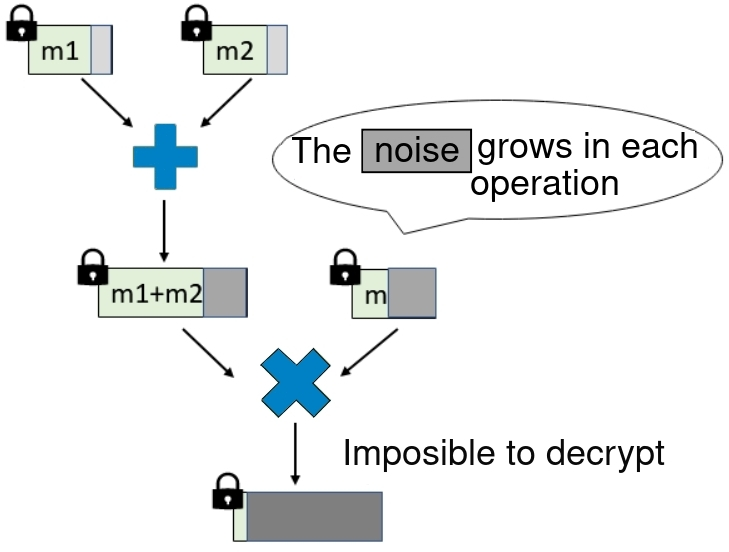
\includegraphics[scale=0.2]{multNoise.jpg}
        \end{figure}

\end{columns}    Fully Homomorphic Encrpytion (FHE): Unlimited number of operations. In this type of schemes
    it use \texttt{Bootstrapping} that are techniques that refresh this error.


\end{frame}
%%%%%%%%%%%%%%%%%%%%%%%%%%%%%%%%%%%%%%%%%%%%%%%%%%%%%%%%%%%%%%%%%%%%%%%%%%%%%%%%%%%%%%%%%%%%%%%%%%%%


\begin{frame}
\frametitle{Bootstrapping}

Bootstrapping vs leveling

o para la siguiente clase?
\end{frame}



%%%%%%%%%%%%%%%%%%%%%%%%%%%%%%%%%%%%%%%%%%%%%%%%%%%%%%%%%%%%%%%%%%%%%%%%%%%%%%%%%%%%%%%%%%%%%%%%%%%%


\begin{frame}
    \frametitle{Schemes}

    Many schemes. \textbf{Warning}: Many acronyms!!!

    Popular schemes by types:
    \begin{itemize}
        \item Operations on integers: BFV and BGV.
        \item Operations on real numbers: CKKS.
        \item Operations on boolean gates: FHEW and THFHE.
    \end{itemize}


    The parameters of all schemes are application-specific and desire security.
\end{frame}

%%%%%%%%%%%%%%%%%%%%%%%%%%%%%%%%%%%%%%%%%%%%%%%%%%%%%%%%%%%%%%%%%%%%%%%%%%%%%%%%%%%%%%%%%%%%%%%%%%%%


\begin{frame}
\frametitle{Math notation}
Most schemes works in a Polynomial Ring domain.

N will be the degree of the Polynomials (N-1).

q and t will be the mod of the coefficients.

\textbf{Ring}: a set with addition, substraction and multiplication. (and other propertys, comutative, associativity, etc).

This operations of elements in a ring return elements in the ring $\rightarrow$ take modulus.




\end{frame}

%%%%%%%%%%%%%%%%%%%%%%%%%%%%%%%%%%%%%%%%%%%%%%%%%%%%%%%%%%%%%%%%%%%%%%%%%%%%%%%%%%%%%%%%%%%%%%%%%%%%


\begin{frame}
\frametitle{Math notation}
BFV, BGV and CKKS works with:    $\mathcal{R}_q =\mathbb{Z}_q[X]/(X^N+1)$

$\mathbb{Z}[X]$ = Set of Polynomials with integer coffiencients.

$\mathbb{Z}_q[X]$ = Set of Polynomials with integer coffiencients mod q.

$\mathbb{Z}_q[X]/(X^N+1)$ = The Polynomials degree N-1.


\end{frame}

%%%%%%%%%%%%%%%%%%%%%%%%%%%%%%%%%%%%%%%%%%%%%%%%%%%%%%%%%%%%%%%%%%%%%%%%%%%%%%%%%%%%%%%%%%%%%%%%%%%%


\begin{frame}
\frametitle{BFV Primitives}

    Basic Primitives (simplified):
\begin{itemize}
    \item ParamGen($\lambda$)$\rightarrow$ Params. Security $\lambda \sim$ $2^\lambda$ operation to decrypt with prob 1.
    \item KeyGen(Params) $\rightarrow$ SK, PK, EvalK
    \item Encrypt(PK, m) $\rightarrow$ c
    \item Decrypt(SK, c) $\rightarrow$ m
    \item EvalAdd(c$_1$, c$_2$) $\rightarrow$ c$_3$
    \item EvalMult(c$_1$, c$_2$) $\rightarrow$ c$_3$
    \item Relinerize(c$_3$, EvalK) $\rightarrow$ c$_3$'
\end{itemize}

\end{frame}

%%%%%%%%%%%%%%%%%%%%%%%%%%%%%%%%%%%%%%%%%%%%%%%%%%%%%%%%%%%%%%%%%%%%%%%%%%%%%%%%%%%%%%%%%%%%%%%%%%%%


\begin{frame}
\frametitle{Workflow}

    Encryption has two phases:
\begin{itemize}
    \item From an integer m to Plaintext
    \item From plain text to ciphertext c.
\end{itemize}


\begin{figure}
    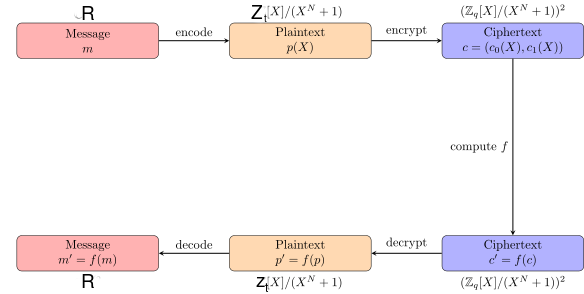
\includegraphics[width=0.85\textwidth]{bfv-diagram.png}
\end{figure}


\end{frame}


%%%%%%%%%%%%%%%%%%%%%%%%%%%%%%%%%%%%%%%%%%%%%%%%%%%%%%%%%%%%%%%%%%%%%%%%%%%%%%%%%%%%%%%%%%%%%%%%%%%%


\begin{frame}
\frametitle{BFV}

The parameters depends in the security level needed and amount of operations that will made.

The parameters depends in the security level needed and amount of operations that will made.



The parameters depends in the security level needed and amount of operations that will made.


Some usual parameters to get the sense of what we are doing:

N = 8192, 16384, 32768.

q = $2^{218}$,   $2^{438}$,  $2^{881}$.

t = less than q.



    \textbf{Implementations}: Residue Number System (RNS) (stay with 64bits arithmetics).

\end{frame}
%%%%%%%%%%%%%%%%%%%%%%%%%%%%%%%%%%%%%%%%%%%%%%%%%%%%%%%%%%%%%%%%%%%%%%%%%%%%%%%%%%%%%%%%%%%%%%%%%%%%


\begin{frame}
\frametitle{Encryption}

Encryption has two phases:

 - From an integer m to Plaintext M $\rightarrow$ Easy, binary representation as Polynomial coefficient.

    - From plaintext to ciphertext using $PK = (PK_1, PK_2)$:

\begin{itemize}
    \item Sample a polynomail $u$ from $\mathcal{R}_2$.
    \item Sample polynomial errors $e_1$ and $e_2$ form a Gaussian distribution.
    \item Calculate $\triangle = \lfloor q/t\rfloor $
    \item Encryption of plaintext M is $C=(C_1, C_2)$
\end{itemize}
\begin{align}
    &C_1 = [PK_1 * u + e_1 + \triangle M ]_q\nonumber \\
    &C_2 = [PK_2 * u + e_2]_q\nonumber
\end{align}


\end{frame}
%%%%%%%%%%%%%%%%%%%%%%%%%%%%%%%%%%%%%%%%%%%%%%%%%%%%%%%%%%%%%%%%%%%%%%%%%%%%%%%%%%%%%%%%%%%%%%%%%%%%


\begin{frame}
\frametitle{Multiplication}

    Multiplication: computation cost and error grow.

    $C_{mul} = C*C' = (C_1*C_1',C_1*C_2'+C_2*C_1', C_2*C_2') = (C_a,C_b,C_c)$

    \textbf{Problem}: If we keep multipling, the number of Polynomials will grow and will be needed
    the squared of the SK.

    \textbf{Relinerize}:
    $EvalK = (-PK_1+SK^2, PK_2)$

    $C_{mul} = (C_a, C_b, C_c)\approx ([C_a+EvalK_1*C_c]_q, [C_b+EvalK_2*C_c]_q)$

    \textbf{Other problem}: we are multiplying the errors of the two ciphertexts, the result error
    grows a lot!
\vspace{-0.1cm}

    \textbf{Solution}: \vspace{-0.3cm}
    \begin{itemize} \vspace{-0.2cm}
        \item Select the lowest parametrs for te exact numbers of operations needed (HE). \vspace{-0.2cm}
        \item Use Bootstrapping us needed (FHE). Even more demanding (multiple multiplications like $C_{mul}$).
    \end{itemize}
\end{frame}
%%%%%%%%%%%%%%%%%%%%%%%%%%%%%%%%%%%%%%%%%%%%%%%%%%%%%%%%%%%%%%%%%%%%%%%%%%%%%%%%%%%%%%%%%%%%%%%%%%%%

\begin{frame}
\frametitle{Recap}

    \textbf{Rembember!} All things are high degree polynomials with huge coeffient.

For a single multiplication of two numbers:
\begin{itemize}
    \item Enconde and encrypt: Sample the errors and parts of the Keys and multiply them to generate the Keys.
    \item Multiplication: Multply the different parts of the ciphertexts.
    \item Relinerize: Multiply the result with the evaluation key.
\end{itemize}

Each homomorphic operation is $10^3 \sim 10^6$ times slower than unencrypted.
\pause

Large footprint in memory.
An encrypted date can occupy $10^5$ more space.

\pause
The schemes are iterative, operating many time with each data.
\pause



\end{frame}
%%%%%%%%%%%%%%%%%%%%%%%%%%%%%%%%%%%%%%%%%%%%%%%%%%%%%%%%%%%%%%%%%%%%%%%%%%%%%%%%%%%%%%%%%%%%%%%%%%%%


\begin{frame}
\frametitle{Research}

\begin{itemize}
   \item Accelerating the polynomial multiplication:
    For these they use Number Theoretic Transform (NTT), a Discreate Fourier Transform (DFT) over a ring.
    \item New schemes.
    \item New upgrades in the schemes (like RNS).
   \item New methods of Bootstrapping.
   \item Software Optimization.
   \item Hardware Acceleration (GPUs, FPGA, specific designs).
\end{itemize}

\end{frame}
%%%%%%%%%%%%%%%%%%%%%%%%%%%%%%%%%%%%%%%%%%%%%%%%%%%%%%%%%%%%%%%%%%%%%%%%%%%%%%%%%%%%%%%%%%%%%%%%%%%%


\begin{frame}
\frametitle{New approach}

    The usual way of approaching this problem of speed (and others):  accelerating the server
    part.

    The new approach:  accelerate the client side.

    CHACO: \textbf{C}lient-aided \textbf{H}E for \textbf{O}paque \textbf{C}ompute \textbf{O}ffloading.


    \begin{itemize}
        \item Another way to operate by using multiple times the client.
        \item New algorithm: rotational redundancy.
        \item Reduction of parameters values.
        \item Minimice client costs.
        \item Hardware acceleration for client: CHACO-TACO
    \end{itemize}


\end{frame}

%%%%%%%%%%%%%%%%%%%%%%%%%%%%%%%%%%%%%%%%%%%%%%%%%%%%%%%%%%%%%%%%%%%%%%%%%%%%%%%%%%%%%%%%%%%%%%%%%%%%

\begin{frame}
\frametitle{FHE requirements and problems:}


\end{frame}

%%%%%%%%%%%%%%%%%%%%%%%%%%%%%%%%%%%%%%%%%%%%%%%%%%%%%%%%%%%%%%%%%%%%%%%%%%%%%%%%%%%%%%%%%%%%%%%%%%%%


\begin{frame}
\frametitle{}


\end{frame}


%%%%%%%%%%%%%%%%%%%%%%%%%%%%%%%%%%%%%%%%%%%%%%%%%%%%%%%%%%%%%%%%%%%%%%%%%%%%%%%%%%%%%%%%%%%%%%%%%%%%


\begin{frame}
\frametitle{}

\end{frame}


%%%%%%%%%%%%%%%%%%%%%%%%%%%%%%%%%%%%%%%%%%%%%%%%%%%%%%%%%%%%%%%%%%%%%%%%%%%%%%%%%%%%%%%%%%%%%%%%%%%%


\end{document}

